\documentclass{beamer}
\mode<presentation>
\usepackage{amsmath,amssymb,mathtools}
\usepackage{textcomp}
\usepackage{gensymb}
\usepackage{adjustbox}
\usepackage{subcaption}
\usepackage{enumitem}
\usepackage{multicol}
\usepackage{listings}
\usepackage{url}
\usepackage{graphicx} % <-- needed for images
\def\UrlBreaks{\do\/\do-}

\usetheme{Boadilla}
\usecolortheme{lily}
\setbeamertemplate{footline}{
  \leavevmode%
  \hbox{%
  \begin{beamercolorbox}[wd=\paperwidth,ht=2ex,dp=1ex,right]{author in head/foot}%
    \insertframenumber{} / \inserttotalframenumber\hspace*{2ex}
  \end{beamercolorbox}}%
  \vskip0pt%
}
\setbeamertemplate{navigation symbols}{}

\lstset{
  frame=single,
  breaklines=true,
  columns=fullflexible,
  basicstyle=\ttfamily\tiny   % tiny font so code fits
}

\numberwithin{equation}{section}

% ---- your macros ----
\providecommand{\nCr}[2]{\,^{#1}C_{#2}}
\providecommand{\nPr}[2]{\,^{#1}P_{#2}}
\providecommand{\mbf}{\mathbf}
\providecommand{\pr}[1]{\ensuremath{\Pr\left(#1\right)}}
\providecommand{\qfunc}[1]{\ensuremath{Q\left(#1\right)}}
\providecommand{\sbrak}[1]{\ensuremath{{}\left[#1\right]}}
\providecommand{\lsbrak}[1]{\ensuremath{{}\left[#1\right.}}
\providecommand{\rsbrak}[1]{\ensuremath{\left.#1\right]}}
\providecommand{\brak}[1]{\ensuremath{\left(#1\right)}}
\providecommand{\lbrak}[1]{\ensuremath{\left(#1\right.}}
\providecommand{\rbrak}[1]{\ensuremath{\left.#1\right)}}
\providecommand{\cbrak}[1]{\ensuremath{\left\{#1\right\}}}
\providecommand{\lcbrak}[1]{\ensuremath{\left\{#1\right.}}
\providecommand{\rcbrak}[1]{\ensuremath{\left.#1\right\}}}
\theoremstyle{remark}
\newtheorem{rem}{Remark}
\newcommand{\sgn}{\mathop{\mathrm{sgn}}}
\providecommand{\abs}[1]{\left\vert#1\right\vert}
\providecommand{\res}[1]{\Res\displaylimits_{#1}}
\providecommand{\norm}[1]{\lVert#1\rVert}
\providecommand{\mtx}[1]{\mathbf{#1}}
\providecommand{\mean}[1]{E\left[ #1 \right]}
\providecommand{\fourier}{\overset{\mathcal{F}}{ \rightleftharpoons}}
\providecommand{\system}{\overset{\mathcal{H}}{ \longleftrightarrow}}
\providecommand{\dec}[2]{\ensuremath{\overset{#1}{\underset{#2}{\gtrless}}}}
\newcommand{\myvec}[1]{\ensuremath{\begin{pmatrix}#1\end{pmatrix}}}
\let\vec\mathbf

\title{Matgeo Presentation - 6.3.3}
\author{ee25btech11063 - Vejith}

\begin{document}


\frame{\titlepage}
\begin{frame}{Question}
Find the shortest distance between the lines given by\\
$\vec{r} = (8 + 3\lambda) \hat{i} - (9 + 16\lambda) \hat{j} + (10 + 7\lambda) \hat{k}$ and $ \vec{r} = 15 \hat{i} + 29 \hat{j} + 5 \hat{k} + \mu (3 \hat{i} + 8 \hat{j} - 5 \hat{k}).$
\end{frame}

\begin{frame}{Solution}
The given lines can be written in vector form as
\begin{align}
    \vec{X}=\myvec{8\\-9\\10}+k\myvec{3\\-16\\7}\\
    \vec{X}=\myvec{15\\29\\5}+k\myvec{3\\8\\-5}\\
    \end{align}
which are of the form
\begin{align}
    \vec{X_1}=\vec{A} + k_1\vec{m_1}\\
    \vec{X_2}=\vec{B} + k_2\vec{m_2}
    \end{align}
     let  $\vec{M}=\brak{\vec{m_1}\hspace{0.5cm}\vec{m_2}}$  and  $\vec{K}=\myvec{k_1\\-k_2}$ be the values of k for which shortest distance between the two lines occurs 
\end{frame}

\begin{frame}{Solution}
    \begin{align}
    \implies \vec{M}=\begin{pmatrix}
    3 & 3\\
    -16 & 8\\
    7 & -5
        \end{pmatrix} \text{ and }\vec{B-A}=\myvec{7\\38\\-5}\\
         \brak{\vec{M} \hspace{0.5cm} \vec{B-A}}=\begin{pmatrix}
            3 & 3 & 7\\
            -16 & 8 & 38\\
            7 & -5 & -5
        \end{pmatrix} \xleftrightarrow{R_2 \rightarrow R_2+\frac{16}{3}\times R_1}
        \begin{pmatrix}
            3 & 3 & 7\\
            0 & 24 & \frac{226}{3}\\
            7 & -5 & -5
        \end{pmatrix}\\
        \xleftrightarrow{R_3 \rightarrow R_3-\frac{7}{3}\times R_1}\begin{pmatrix}
            3 & 3 & 7\\
            0 & 24 & \frac{226}{3}\\
            0 & -12 & -\frac{64}{3}
        \end{pmatrix}\\
        \xleftrightarrow{R_3 \rightarrow R_3+\frac{1}{2}\times R_2} \begin{pmatrix}
            3 & 3 & 7\\
            0 & 24 & \frac{226}{3}\\
            0 & 0 & -\frac{49}{3}
        \end{pmatrix}
\end{align}
The above matrix now is in row echelon form.Rank of a matix in echelon form is number of non zero rows.so,The rank of the above  matrix is 3
\end{frame}

\begin{frame}{Solution}
$\implies$ given lines are skew.
\begin{align}
\implies \vec{M}^T\vec{M}\vec{K}=\vec{M}^T\brak{\vec{B}-\vec{A}}\\
    \begin{pmatrix}
        3 & -16 & 7\\
        3 & 8 & -5
    \end{pmatrix}\begin{pmatrix}
    3 & 3\\
    -16 & 8\\
    7 & -5
        \end{pmatrix}\vec{K}=\begin{pmatrix}
        3 & -16 & 7\\
        3 & 8 & -5
    \end{pmatrix}\myvec{7\\38\\-5}\\
    \implies \begin{pmatrix}
        314 & -154\\
        -154 & 98
    \end{pmatrix}\vec{K}=\myvec{-622\\350}
\end{align}
The augmented matrix of above equation is given by
\begin{align}
    \left(\begin{array}{cc|c}
        314 & -154 & -622 \\
        -154 & 98 & 350 
\end{array}\right) &\xleftrightarrow{R_1 \rightarrow R_1+ 2R_2} \left(\begin{array}{cc|c}
        6 & 42 & 78 \\
        -154 & 98 & 350 
\end{array}\right)\\ &\xleftrightarrow{R_2 \rightarrow R_2+ \frac{77}{3}\times R_2} \left(\begin{array}{cc|c}
        6 & 42 & 78 \\
        0 & 1176 & 2352 
\end{array}\right)\\
&\xleftrightarrow{R_1 \rightarrow \frac{1}{6}\times R_1} \left(\begin{array}{cc|c}
        1 & 7 & 13 \\
        0 & 1176 & 2352 
\end{array}\right)\\
\text{On back substitution we get, } 
\end{align}
\end{frame}
\begin{frame}{Conclusion}
    \begin{align}
\vec{K}=\myvec{k_1\\-k_2}=\myvec{-1\\2}
\end{align}

\begin{align}
    \implies \vec{X_1}=\myvec{5\\7\\3} \text{ and }\vec{X_2}=\myvec{9\\13\\15}\\
\end{align}
The minimum distance between the lines is given by
\begin{align}
    \norm{\vec{X_2-X_1}}=\norm{\myvec{4\\6\\12}}=14
\end{align} 
\end{frame}

\begin{frame}{Plot}
    \begin{figure}[h!]
    \centering
    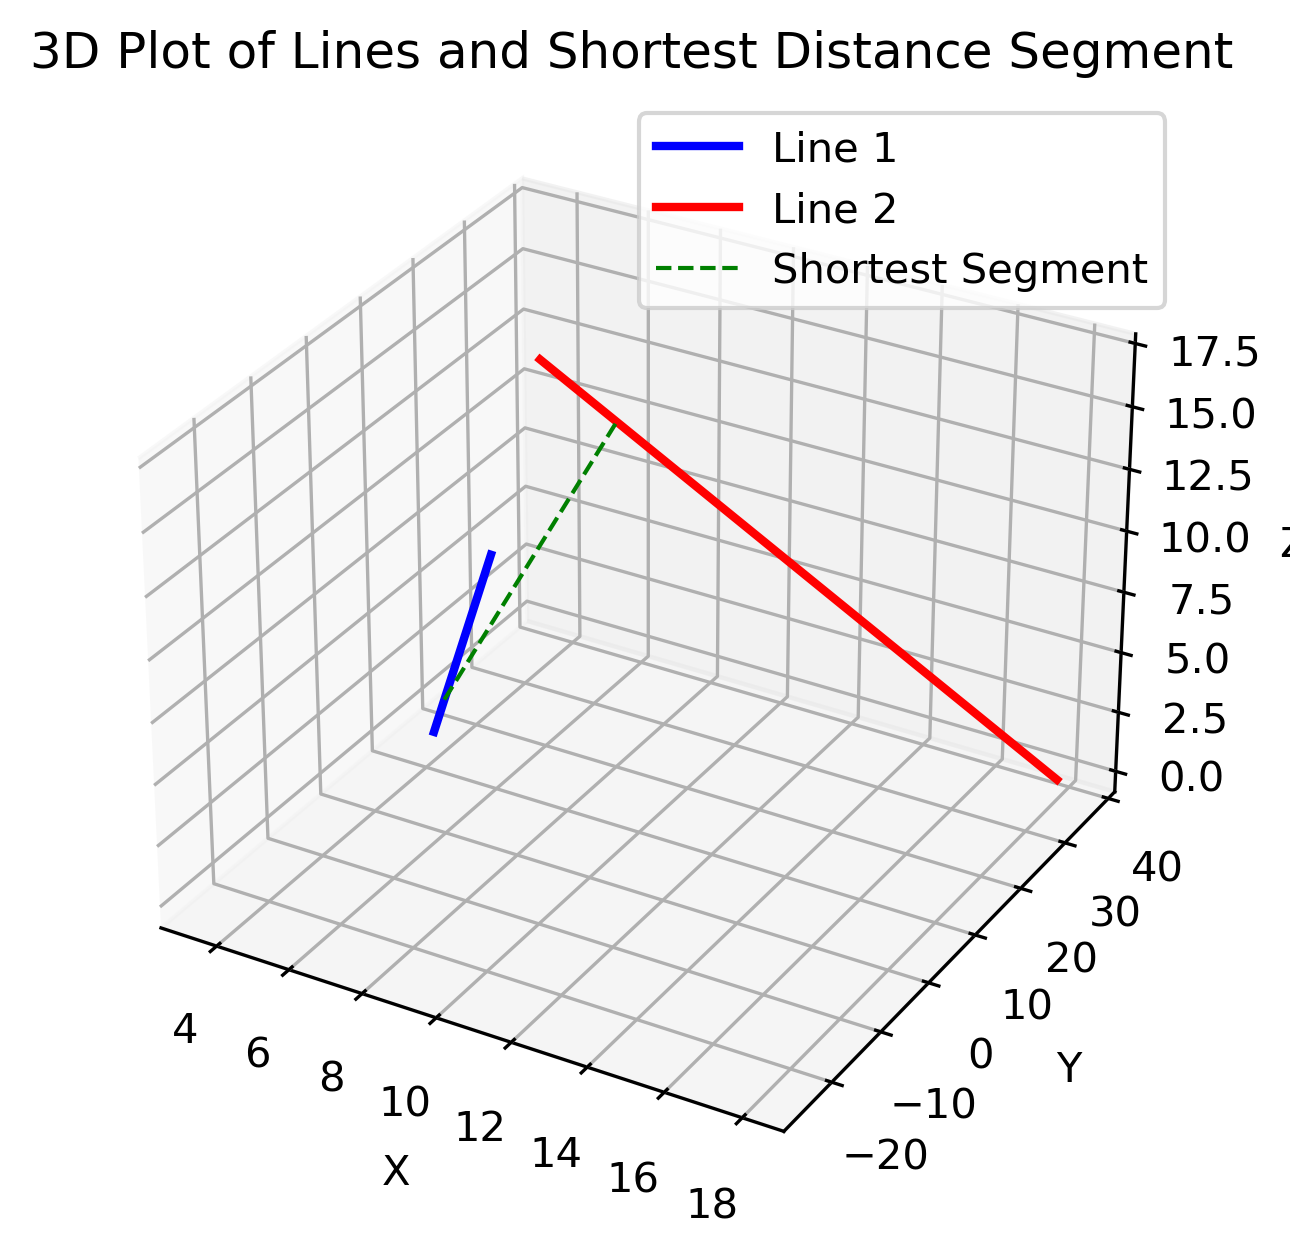
\includegraphics[width=0.6\columnwidth]{figs/01.png}
    \caption{Caption}
    \label{fig:placeholder}
\end{figure}
\end{frame}

% --------- CODE APPENDIX ---------
\section*{Appendix: Code}

% C program
\begin{frame}[fragile]{C Code: line.c}
\begin{lstlisting}[language=C]
#include <stdio.h>

int main() {
    #include <stdio.h>
#include <math.h>

int main() {
    // Define P1, d1, P2, d2
    double P1[3] = {8, -9, 10};
    double d1[3] = {3, -16, 7};
    double P2[3] = {15, 29, 5};
    double d2[3] = {3, 8, -5};

    // Compute c = P1 - P2
    double c[3];
    for (int i = 0; i < 3; i++) {
        c[i] = P1[i] - P2[i];
    }

    // Matrix M = [d1  -d2]
    double M[3][2] = {
        { d1[0], -d2[0] },
        { d1[1], -d2[1] },
        { d1[2], -d2[2] }
    };

    // Compute M^T * M (2x2 matrix)
    double MTM[2][2] = {0};
    for (int i = 0; i < 2; i++) {
        for (int j = 0; j < 2; j++) {
            for (int k = 0; k < 3; k++) {
                MTM[i][j] += M[k][i] * M[k][j];
            }}}
\end{lstlisting}
\end{frame}

\begin{frame}[fragile]{C Code: line.c}
\begin{lstlisting}[language=C]
    // Compute -M^T * c (2x1 vector)
    double rhs[2] = {0};
    for (int i = 0; i < 2; i++) {
        for (int k = 0; k < 3; k++) {
            rhs[i] -= M[k][i] * c[k];
        }
    }

    // Solve 2x2 linear system MTM * x = rhs
    double det = MTM[0][0]*MTM[1][1] - MTM[0][1]*MTM[1][0];
    double lambda = ( rhs[0]*MTM[1][1] - rhs[1]*MTM[0][1] ) / det;
    double mu     = ( MTM[0][0]*rhs[1] - MTM[1][0]*rhs[0] ) / det;

    // Closest points Q1 and Q2
    double Q1[3], Q2[3];
    for (int i = 0; i < 3; i++) {
        Q1[i] = P1[i] + lambda * d1[i];
        Q2[i] = P2[i] + mu * d2[i];
    }
    // Distance = ||Q1 - Q2||
    double dx = Q1[0] - Q2[0];
    double dy = Q1[1] - Q2[1];
    double dz = Q1[2] - Q2[2];
    double distance = sqrt(dx*dx + dy*dy + dz*dz);

    // Write result to file "line.dat"
    FILE *fp = fopen("line.dat", "w");
    if (fp == NULL) {
        printf("Error opening file!\n");
        return 1;}
    fprintf(fp, "Shortest distance between the lines = %.2f\n", distance);
    fclose(fp);
return 0;}
\end{lstlisting}
\end{frame}

\begin{frame}[fragile]{Python: plot.py}
\begin{lstlisting}[language=Python]
import numpy as np
import matplotlib.pyplot as plt
from mpl_toolkits.mplot3d import Axes3D

# Parameter ranges
lambda_vals = np.linspace(-1.5, 1, 100)
mu_vals = np.linspace(-2.5, 1, 100)

# Line 1: r = (8 + 3λ) i - (9 + 16λ) j + (10 + 7λ) k
x1 = 8 + 3 * lambda_vals
y1 = -9 - 16 * lambda_vals
z1 = 10 + 7 * lambda_vals

# Line 2: r = 15i + 29j + 5k + μ(3i + 8j - 5k)
x2 = 15 + 3 * mu_vals
y2 = 29 + 8 * mu_vals
z2 = 5 - 5 * mu_vals

fig = plt.figure()
ax = fig.add_subplot(111, projection='3d')

# Plot Line 1
ax.plot(x1, y1, z1, label='Line 1', color='blue', linewidth=2)

# Plot Line 2
ax.plot(x2, y2, z2, label='Line 2', color='red', linewidth=2)

# Shortest distance segment as thin dashed green line
S1 = np.array([5., 7., 3.])
S2 = np.array([9., 13., 15.])
ax.plot([S1[0], S2[0]], [S1[1], S2[1]], [S1[2], S2[2]],
        color='green', linestyle='--', linewidth=1, label='Shortest Segment')
\end{lstlisting}
\end{frame} 

\begin{frame}[fragile]{Python: plot.py}
\begin{lstlisting}[language=Python]
# Axes labels and legend
ax.set_xlabel('X')
ax.set_ylabel('Y')
ax.set_zlabel('Z')
ax.legend()
ax.set_title('3D Plot of Lines and Shortest Distance Segment')
plt.savefig('shortest_distance_3d.png', dpi=300, bbox_inches='tight')
plt.show()

\end{lstlisting}
\end{frame} 
\end{document}
